\documentclass{article}
\usepackage{forloop}
\usepackage{rotating}
\usepackage{subcaption}
\usepackage{array}

\newcounter{row}  
\newcounter{col}


\begin{document}
% this is your table (minimal example)
\begin{figure}
\begin{tabular}{ m{1em} || c c c}  
  \forloop{row}{1}{\value{row} < 9}{
    \begin{sideways}{Renglon \arabic{row}}\end{sideways} 
    \forloop{col}{1}{\value{col} < 4}{
      & \begin{subfigure}[b]{0.35\textwidth}  
          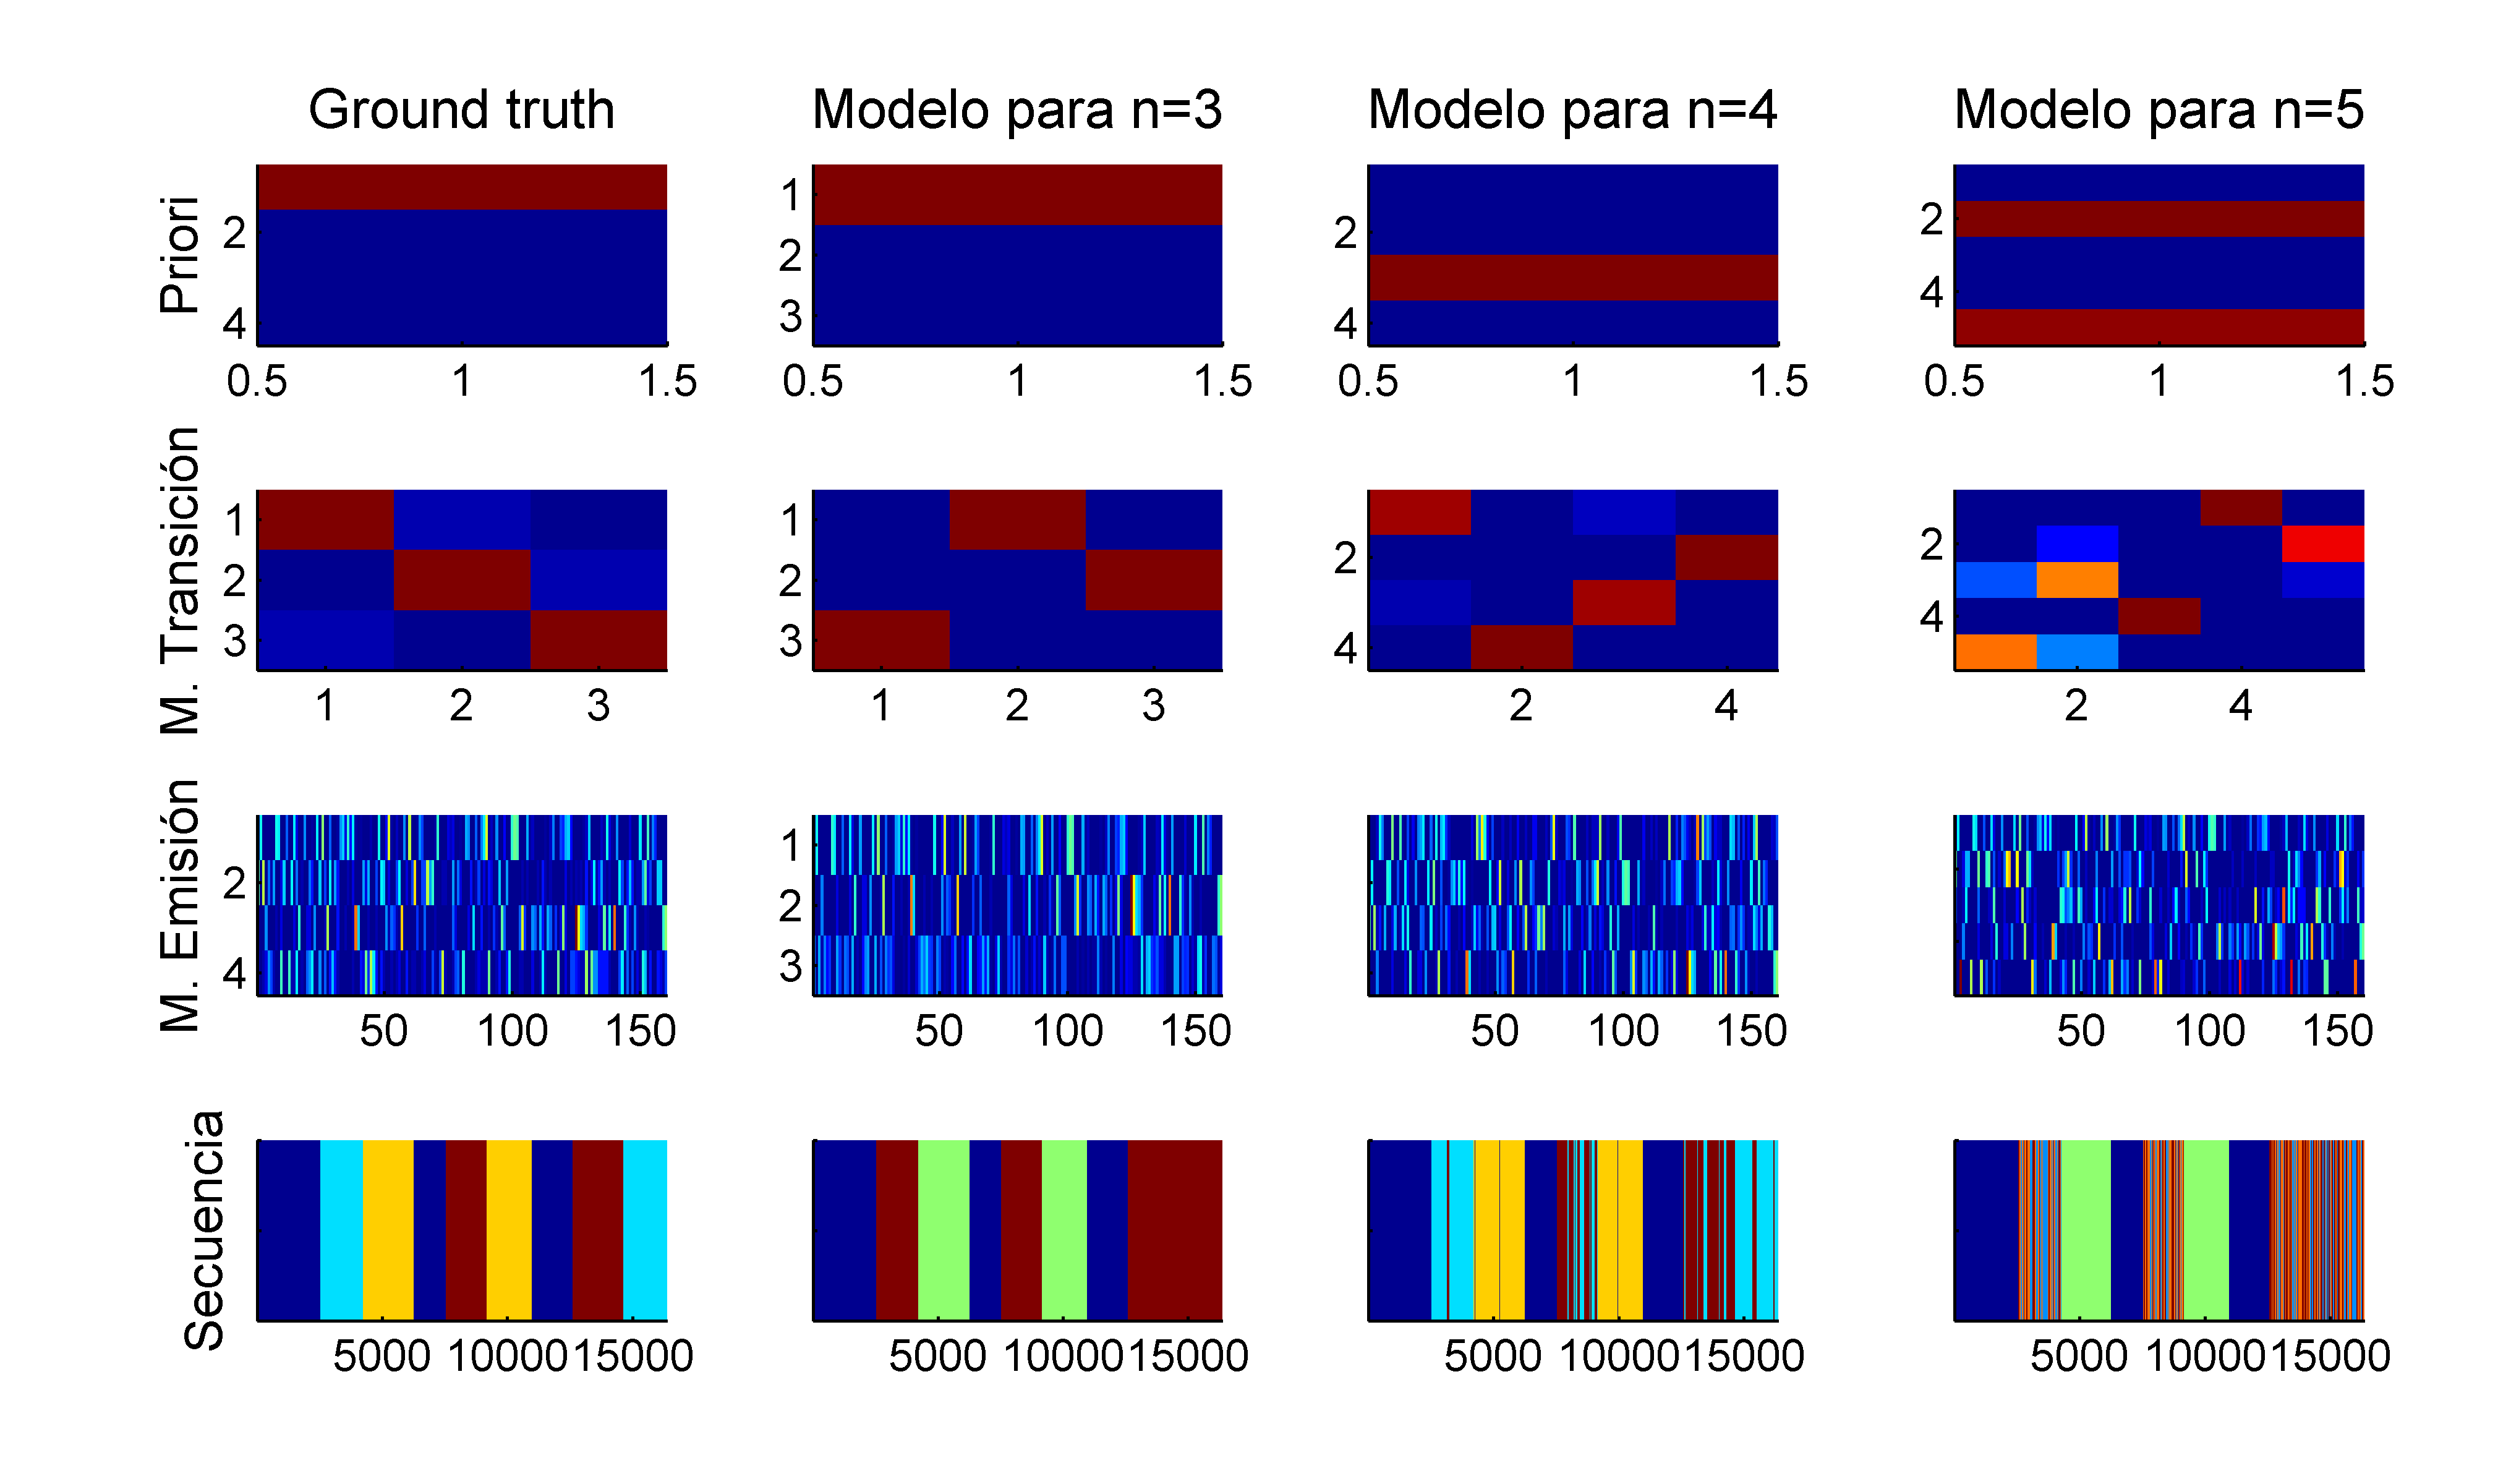
\includegraphics[width=1\textwidth]{gfx/chap6/lear31}        
        \end{subfigure}
        }
    \\ \hline
  }   
\end{tabular}
\end{figure}


\end{document}